% vim:autoindent:set textwidth=78:

\section{Compositore di stampe}\label{label_printcomposer}

% when the revision of a section has been finalized, 
% comment out the following line:
% \updatedisclaimer

Il compositore di stampe fornisce funzionalità per la creazione di layout di
stampa che saranno continuamente migliorate. Consente di aggiungere elementi
al layout come la vista mappa, la legenda, la barra di scala, immagini esterne
e campi testuali. È possibile cambiare le dimensioni, raggruppare e spostare
ogni elemento e regolarne le proprietà per creare il layout desiderato. 
Il risultato può essere stampato (anche come Postscript e PDF), esportato come
immagine o come disegno vettoriale in formato SVG.\footnote{L'esportazione in
SVG è supportata, ma non funziona correttamente con alcune recenti versioni di
QT4. È necessario fare delle prove e dei controlli individuali sul proprio
sistema} Si veda l'elenco degli strumenti nella tabella~\ref{tab:printcomposer_tools}:

\begin{table}[h]\index{Print composer!tools}
\centering
\caption{Strumenti del compositore di stampe}\label{tab:printcomposer_tools}\medskip
 \begin{tabular}{|l|p{6.9cm}|l|p{6.9cm}|}
 \hline \textbf{Icona} & \textbf{Scopo} & \textbf{Icona} &
 \textbf{Scopo} \\

 \hline 
\includegraphics[width=0.7cm]{mActionExportMapServer}
 & Esporta come immagine & 
 
\includegraphics[width=0.7cm]{mActionSaveAsSVG} & Esporta come SVG \\
 \hline 
\includegraphics[width=0.7cm]{mActionFilePrint} & Stampa o esporta
 come PDF o Postscript &
 
\includegraphics[width=0.7cm]{mActionZoomFullExtent} & Zoomma all'estensione
 massima \\
 \hline 
\includegraphics[width=0.7cm]{mActionZoomIn} & Ingrandisci &
 
\includegraphics[width=0.7cm]{mActionZoomOut} & Rimpicciolisci \\
 \hline 
\includegraphics[width=0.7cm]{mActionDraw} & Aggiorna la vista &
 
\includegraphics[width=0.7cm]{mActionAddRasterLayer} & Aggiungi una nuova
 vista mappa da QGIS \\
 \hline 
\includegraphics[width=0.7cm]{mActionSaveMapAsImage} & Aggiungi
 immagine al layout di stampa &
 
\includegraphics[width=0.7cm]{mActionLabel} & Aggiungi caselle di testo al
 layout di stampa \\
 \hline 
\includegraphics[width=0.7cm]{mActionAddLegend} & Aggiungi una nuova
 legenda al layout di stampa & 
 
\includegraphics[width=0.7cm]{mActionScaleBar} & Aggiungi una barra di scala
 al layout di stampa\\
 \hline 
\includegraphics[width=0.7cm]{mActionSelectPan} & Seleziona/sposta
 oggetti del layout di stampa &
 
\includegraphics[width=0.7cm]{mActionMoveItemContent} & Sposta centro della
 vista mappa \\
 \hline 
\includegraphics[width=0.7cm]{mActionGroupItems} & Raggruppa oggetti
 del layout & 
 
\includegraphics[width=0.7cm]{mActionUngroupItems} & Separa oggetti del
 layout \\
 \hline 
\includegraphics[width=0.7cm]{mActionRaiseItems} & Alza di livello
 l'oggetto selezionato nel layout &
 
\includegraphics[width=0.7cm]{mActionLowerItems} & Abbassa di livello
 l'oggetto selezionato nel layout \\
 \hline 
\includegraphics[width=0.7cm]{mActionMoveItemsToTop} & Porta l'oggetto
 selezionato in primo piano & 
 
\includegraphics[width=0.7cm]{mActionMoveItemsToBottom} & Porta l'oggetto
 selezionato sullo sfondo \\
\hline
\end{tabular}
\end{table}

Per accedere al compositore di stampe, cliccare sul pulsante
\toolbtntwo{mActionFilePrint}{Print} nella barra strumenti o scegliere la voce
di menù \mainmenuopt{File} > \dropmenuopttwo{mActionFilePrint}{Compositore
stampe}.

\subsection{Uso del compositore di stampe}\label{label_useprintcomposer} 

Prima di iniziare a lavorare con il compositore di stampe, è necessario
caricare alcuni livelli raster e vettoriali nella vista mappa di QGIS e
regolarne le proprietà secondo le proprie esigenze. Una volta effettuate
tutte le impostazioni e applicata la simbologia cliccare sul pulsante
\toolbtntwo{mActionFilePrint}{Compositore stampe}.

\begin{figure}[ht]
   \begin{center}
   \caption{Compositore di stampe \nixcaption}\label{fig:print_composer_blank}\smallskip
   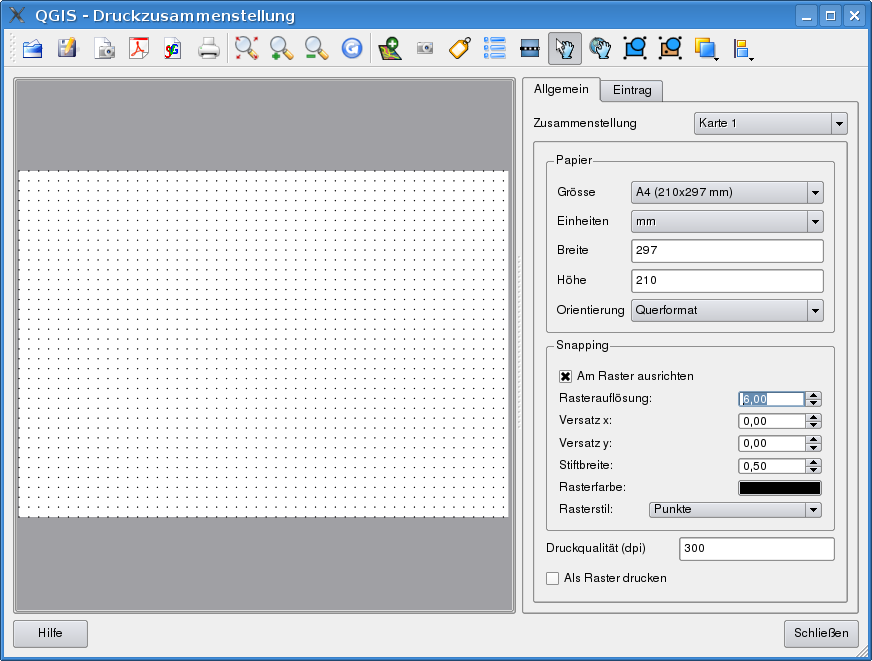
\includegraphics[clip=true, width=\textwidth]{print_composer_blank}
\end{center}  
\end{figure}

Aprendo il compositore di stampe viene visualizzato un foglio bianco al quale
aggiungere vista mappa, legenda, barra di scala, immagini e testo. La Figura
\ref{fig:print_composer_blank} mostra la vista iniziale del compositore di
stampe prima dell'aggiunta di un qualunque elemento. Nel compositore di stampe
co sono due linguette:

\begin{itemize}
\item La linguetta \tab{Generale} consente di impostare la dimensione del
foglio, l'orientamento e la qualità di stampa del file in uscita in dpi.
\item La linguetta \tab{Oggetto} mostra le proprietà dell'elemento selezionato
nel layout di stampa. 
Cliccare sull'icona \toolbtntwo{mActionSelectPan}{Seleziona/Sposta oggetto} 
per selezionare un elemento (ad es. legenda, barra di scala o etichetta
testuale) nel layout. Cliccare dunque sulla linguetta \tab{Oggetto} e
personalizzare le impostazioni dell'elemento selezionato.
\end{itemize}

Possono essere aggiunti diversi elementi al compositore ed è anche
possibile avere più di una vista mappa o legenda o barra di scala nel layout
di stampa. Ogni elemento ha le sue proprietà e, nel caso delle viste mappa, la
propria estensione.

\subsubsection{Aggiungere una vista mappa al layout nel compositore di
stampe}

Per aggiungere una vista mappa, cliccare sul pulsante
\toolbtntwo{mActionAddRasterLayer}{Aggiungi nuova mappa} nella barra strumenti
del compositore di stampe e trascinare il mouse per definire un rettangolo
nell'area occupata dal foglio tenendo premuto il tasto sinistro per aggiungere
la vista mappa. Verrà visualizzato un riquadro vuoto con la scritta
\textit{"La mappa verrà stampata qui"}. Per visualizzare effettivamente la mappa,
selezionare \selectstring{Anteprima}{Cache} nella linguetta \tab{Oggetto}.

\begin{figure}[ht]
\centering
\caption{Print Composer map item tab content \nixcaption}\label{fig:print_composer_map_item}
   \subfigure[Width, height and extend dialog] {\label{subfig:print_composer_map_item1}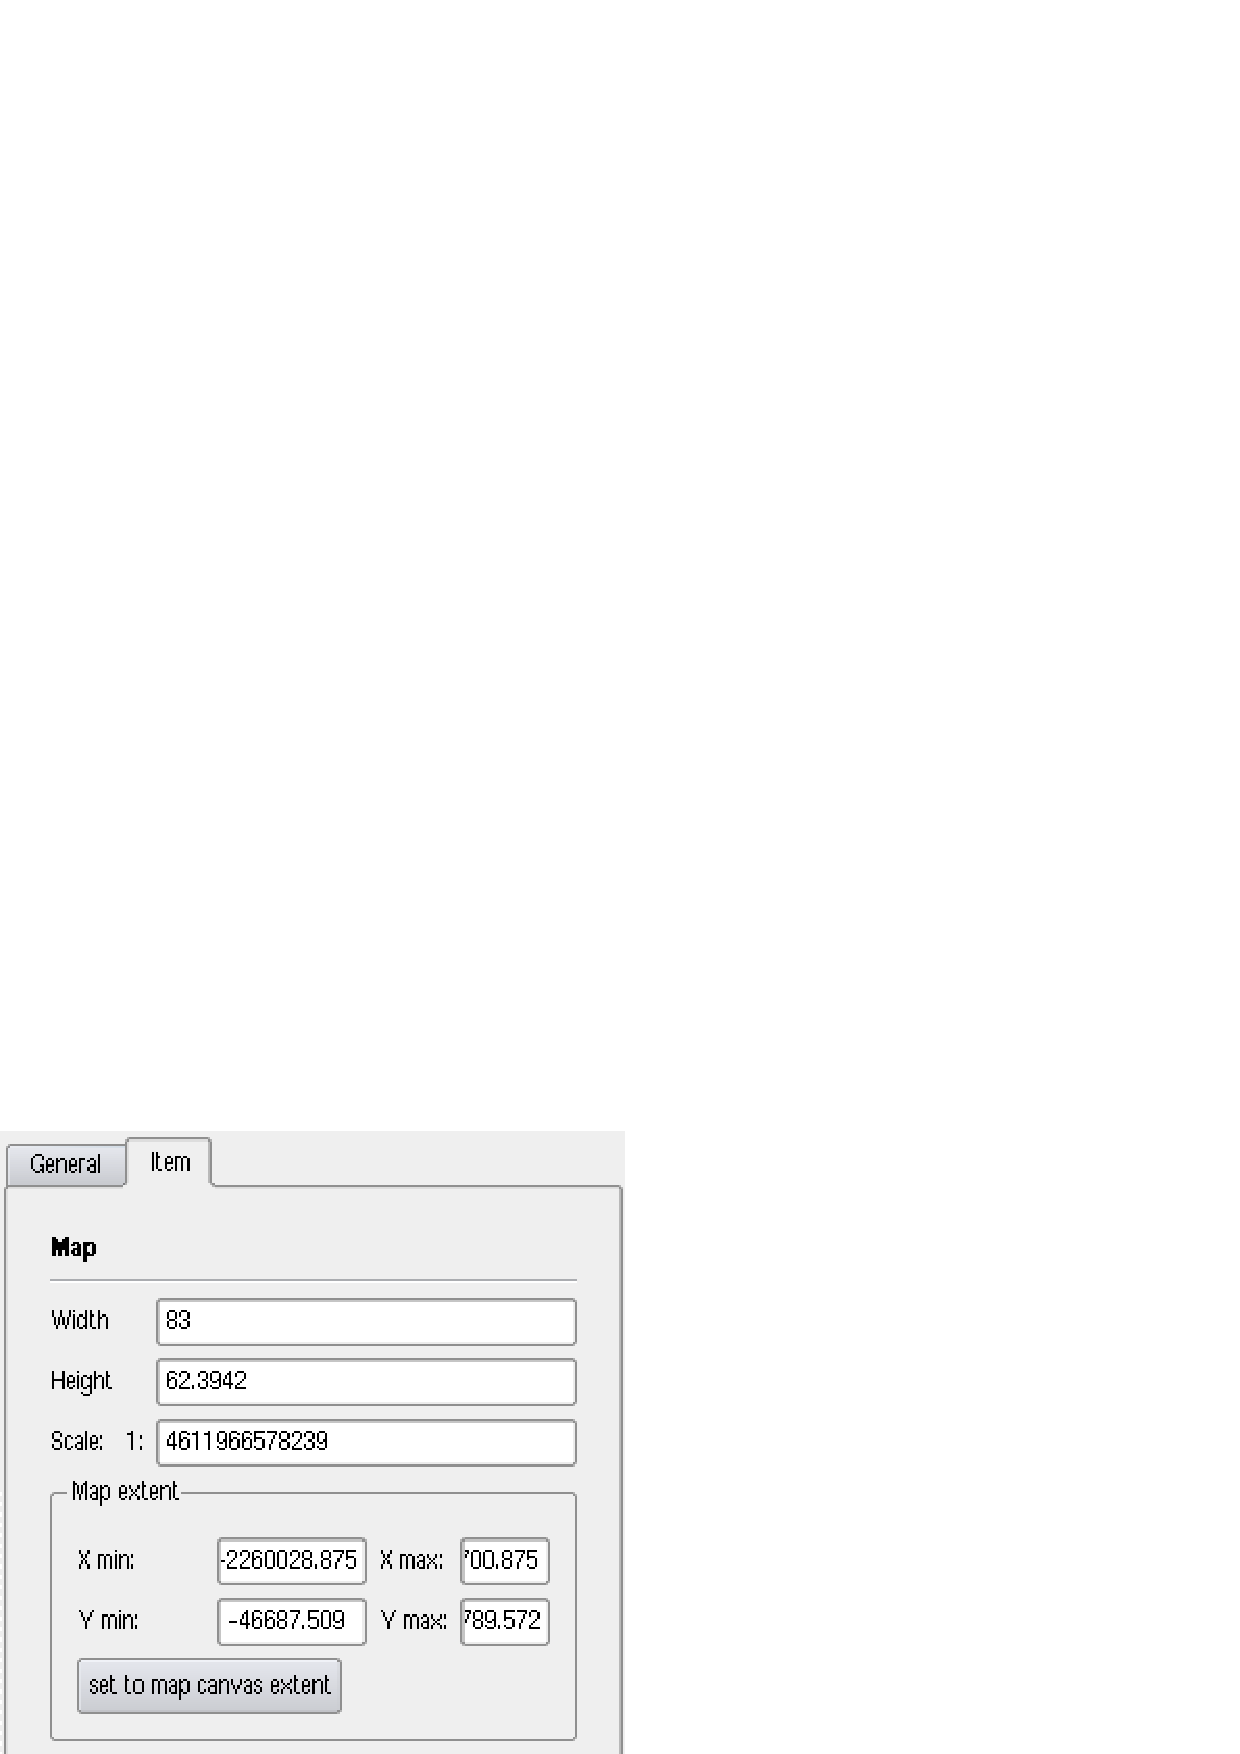
\includegraphics[clip=true, width=0.4\textwidth]{print_composer_map_item1}}\goodgap
   \subfigure[Properties dialog] {\label{subfig:print_composer_map_item2}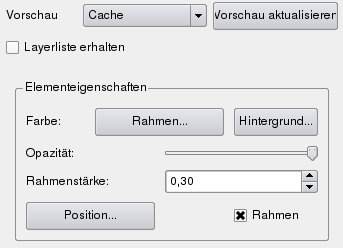
\includegraphics[clip=true, width=0.4\textwidth]{print_composer_map_item2}}
\end{figure}

You can resize the map later by clicking on the \toolbtntwo{mActionSelectPan}{Select/Move item} 
button, selecting the element, and dragging one of the blue handles in the corner of the map. With the 
map selected, you can now adapt more properties in the map \tab{Item} tab. Resize the map 
item specifying the width and height or the scale. Define the map extend using Y and 
X min/max values or clicking the \button{set to map canvas extend} button. Update the 
map preview and select, whether to see a preview from cache or an empty rectangle with 
a \textit{"Map will be printed here"} message. Define colors and outline width for the 
element frame, set a background color and opacity for the map canvas. And you can also 
select or unselect to display an element frame with the \checkbox{frame} checkbox 
(see Figure~\ref{fig:print_composer_map_item}). If you change the view on the QGIS 
map canvas by zooming or panning or changing vector or raster properties, you can 
update the print composer view selecting the map element in the print composer and clicking 
the \button{Update Preview} button in the map \tab{Item} tab 
(see Figure~\ref{fig:print_composer_map_item}). 

To move layers within the map element select the map element, click 
the \toolbtntwo{mActionMoveItemContent}{Move item content} icon 
and move the layers within the map element frame with the left mouse button.

\begin{Tip}\caption{\textsc{Saving a print composer layout}}
\qgistip{If you want to save the current state of a print composer session, click 
on \mainmenuopt{File} > \dropmenuopttwo{mActionFileSaveAs}{Save Project As} to save 
the state of your workspace including the state of the current print composer session. 
It is planned but currently not possible to save print composer templates itself.
}
\end{Tip} 

\subsubsection{Adding other elements to the Print Composer} 

Besides adding a current QGIS map canvas to the Print Composer, it is also possible 
to add, move and customize legend, scalebar, images and label elements.

\minisec{Label and images}

To add a label or an image, click the \toolbtntwo{mActionLabel}{Add label} or 
\toolbtntwo{mActionSaveMapAsImage}{Add image} icon and place the element 
with the left mouse button on the print composer canvas.

\begin{figure}[ht]
\centering
\caption{Customize print composer label and images \nixcaption}\label{fig:print_composer_tab2}
   \subfigure[label item tab] {\label{subfig:print_composer_label_item}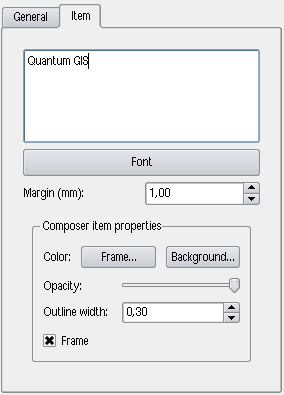
\includegraphics[clip=true, width=0.4\textwidth]{print_composer_label_item}}\goodgap
   \subfigure[image item tab] {\label{subfig:print_composer_image_item}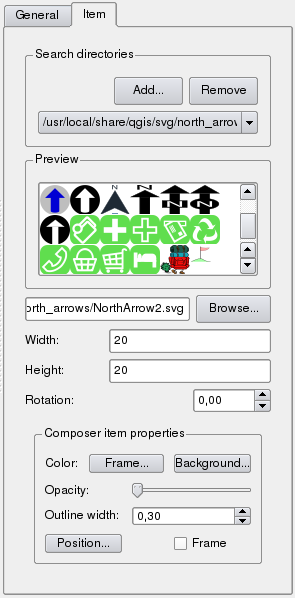
\includegraphics[clip=true, width=0.4\textwidth]{print_composer_image_item}}
\end{figure}

\minisec{Legend and scalebar}

To add a map legend or a scalebar, click the \toolbtntwo{mActionAddLegend}{Add new legend} or 
\toolbtntwo{mActionScaleBar}{Add new scalebar} icon and place the element with the left 
mouse button on the print composer canvas.

\begin{figure}[ht]
\centering
\caption{Customize print composer legend and scalebar \nixcaption}\label{fig:print_composer_tab1}
   \subfigure[legend item tab] {\label{subfig:print_composer_legend_item}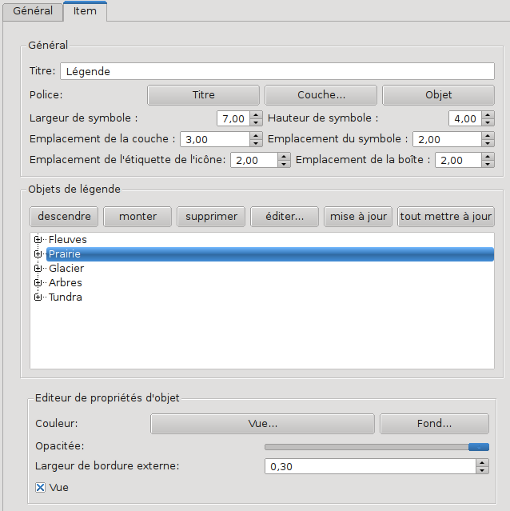
\includegraphics[clip=true, width=0.4\textwidth]{print_composer_legend_item}}\goodgap
   \subfigure[scalebar item tab] {\label{subfig:print_composer_scalebar_item}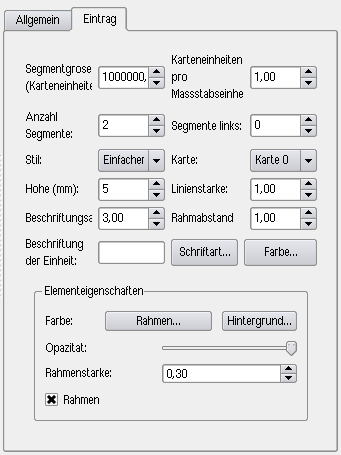
\includegraphics[clip=true, width=0.4\textwidth]{print_composer_scalebar_item}}
\end{figure}

\subsubsection{Navigation tools}

For map navigation the print composer provides 4 general tools:

\begin{itemize}
\item \toolbtntwo{mActionZoomOut}{Zoom in},
\item \toolbtntwo{mActionZoomOut}{Zoom out},
\item \toolbtntwo{mActionZoomFullExtent}{Zoom to full extend} and
\item \toolbtntwo{mActionDraw}{Refresh the view}, if you find the view in an inconsistent state. 
\end{itemize}

\subsubsection{Creating Output}

Figure \ref{fig:print_composer_complete} shows the print composer with an example 
print layout including each type of map element described in the sections above.

\begin{figure}[h]
   \begin{center}
   \caption{Print Composer with map view, legend, scalebar, and text added \nixcaption}
   \label{fig:print_composer_complete}\smallskip
   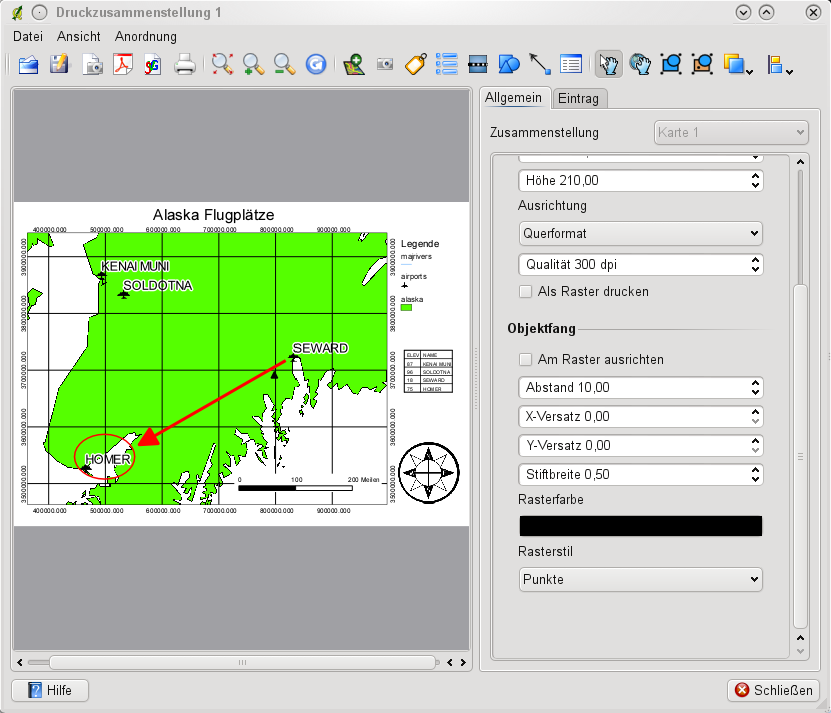
\includegraphics[clip=true, width=\textwidth]{print_composer_complete}
\end{center}  
\end{figure}

The print composer allows you to create several output formats and it is possible to 
define the resolution (print quality) and paper size:

\begin{itemize}
\item The \toolbtntwo{mActionFilePrint}{Print} icon allows to print the layout 
to a connected printer or as PDF or Postscript file depending on installed printer 
drivers.
\item The \toolbtntwo{mActionExportMapServer}{Export as image} icon exports the 
composer canvas in several image formats such as PNG, BPM, TIF, JPG, \dots
\item The \toolbtntwo{mActionSaveAsSVG}{Export as SVG} icon saves the print 
composer canvas as a SVG (Scalable Vector Graphic). \textbf{Note:} Currently the 
SVG output is very basic. This is not a QGIS problem, but a problem of the underlaying 
Qt library. This will hopefully be sorted out in future versions.
\end{itemize}

